\documentclass[12pt]{article}
\usepackage{zed-csp}
\usepackage[top=2.5cm, bottom=2.5cm, left=3cm, right=3cm]{geometry}
\usepackage{graphicx}
\usepackage{subcaption}

\begin{document}

\begin{Huge}
\begin{center}
\begin{normalsize}
\textbf{MAKERERE 
\includegraphics[scale=0.5]{logo} UNIVERSITY }\\

\textbf{SCHOOL OF COMPUTING AND INFORMATICS TECHNOLOGY} \\
\textbf{DEPARTMENT OF COMPUTER SCIENCE} \\
\textbf{BACHELOR OF SCIENCE IN COMPUTER SCIENCE} \\
\textbf{YEAR 2} \\
\textbf{BIT 2207 RESEARCH METHODOLOGY} \\
\textbf{Course Work: Assignment }
\end{normalsize}
\end{center}
\end{Huge}

\begin{center}
\begin{tabular}{|l|l|l|c|}
\hline NAME  & REG NO & STD NO \\\hline
ABILA JOSHUA& 16/U/19130/PS & 216021700 \\\hline
OJOK ISAAC& 16/U/20048/PS& 216021703 \\\hline
LUYIMA SHAFIC& 16/U/6725/PS	 & 216013602 \\\hline
KAGAME STEVENLUC&16/U/5127/PS  & 216012220\\\hline

\end{tabular}

\paragraph{•}
Lecturer:DR. ERNEST MWEBAZE \\


\end{center}

\newpage

\begin{center}
\textbf{\sc Automated monitoring of Ambiguous  street parking dues .}\\
\end{center}

\section{INTRODUCTION}
\paragraph{•}
This document proposes the development of an automated monitoring of Ambiguous street parking bills .The system shall focus on how car owners will access their street parking dues ,in a clear summarised but well organised form .This shall erase any Suspicion, as all the information shall be at their(car owners) exposal .
  
\section{BACKGROUND}
\paragraph{•}
Multiplex Limited Uganda is a private civil construction company and street ticket parking company. Multiplex Limited records information about cars parked on kampala streets, stores the data collections in a database that can be accessed by their cilents from their offices or use mobile phones through mobile money that only shows the a specific block amount to be paid. This could result into denial of payment or furiously storming multiplex offices in need of knowing ,the ambiguous accumulation of parking dues .Generally causing inconveniences to car owners and multiplex officers ,in the struggle to explain accumulation of dues or the reason for having clumped a car .

\subsection{Problem statement} 
Continuous doubt in bills to foot accumulated due to street parking, leaves a lot of car owners with in Kampala disenfranchised from access to clear reports by Multiplex Limited. This arises from current poor report generation, which lacks the ingredient to convince defaulters with a breakdown summary of how the total amount due arises. A remedy to monitor bills would rather erase ambiguity with this current system.

\subsection{Scope}
\paragraph{•}
The development of a web based database that will capture parking details, provide data security, help administrators to monitor bills, give online guidance on how to pay their bills for car owners parking on Kampala streets.

\subsection{General objective}
\paragraph{•}
The main goal of this project is to make it, swift and efficient for all users of the system monitor bills arising from parking on Kampala streets

 
\subsection{Specific Objective}
\paragraph{•}
•	To locate all areas where parking of vehicles can take place and have agents recording number plate of any car that is parking.\\
\paragraph{•}
•	To make sure every time a record is made by the agent, the car owner gets notified through SMS. The SMS should include location, duration of parking and amount he has been charged.\\
\paragraph{•}
•	To make payment as easy as possible using cash or through mobile money.

\subsection{Significance of study}
\paragraph{•}
 Save time by reducing the downtime involved queueing up to check bills. Aswell enable comfort and convenience of accessing parking dues from anywhere at any time.

\section{LITERATURE REVIEW}
\subsubsection {smart parking}
\paragraph{•}
Drivers searching for parking are estimated to be responsible for about 30percent of traffic congestion in cities. Historically, cities, businesses, and property developers have tried to match parking supply to growing demand for parking spaces. It has become clear, though, that simply creating more parking spaces is not sufficient to address the problem of congestion. New approaches using smart parking systems look to provide a more balanced view of parking that better manages the relationship between supply and demand. 
Smart parking can be defined as the use of advanced technologies for the efficient operation, monitoring, and management of parking within an urban mobility strategy. The global market for smart parking systems reached 93.5 million dollars , with the United States representing 46percent market share, and offering a strong growth opportunity for companies offering services in the United States and overseas. A number of technologies provide the basis for smart parking solutions, including vehicle sensors, wireless communications, and data analytics. Smart parking is also made viable by innovation in areas such as smartphone apps for customer services, mobile payments, and in-car navigation systems. At the heart of the smart parking concept is the ability to access, collect, analyze, disseminate, and act on information on parking usage. Increasingly, this information is provided in real-time from intelligent devices that enable both parking managers and drivers to optimize the use of parking capacity. 
i- Motivation to use Smart parking:  
ii. Reduced traffic – Traffic flow increases as fewer cars are required to drive around in search of an open parking space. 
iii. Reduced pollution – Searching for parking burns around one million barrels of oil a day. An optimal parking solution will significantly decrease driving time, thus lowering the amount of daily vehicle emissions and ultimately reducing the global environmental footprint. 
iv. Enhanced User Experience – A smart parking solution will integrate the entire user experience into a unified action. Driver’s payment, spot identification, location search and time notifications all seamlessly become part of the destination arrival process. 
v. New Revenue Streams – Many new revenue streams are possible with smart parking technology. For example, lot owners can enable tiered payment options dependent on parking space location. Also, reward programs can be integrated into existing models to encourage repeat users. 
vi. Integrated Payments and POS – Returning users can replace daily, manual cash payments with account invoicing and application payments from their phone. This could also enable customer loyalty programs and valuable user feedback. 
vii. Increased Safety – Parking lot employees and security guards contain real-time lot data that can help prevent parking violations and suspicious activity. License plate recognition cameras can gather pertinent footage. Also, decreased spot- searching traffic on the streets can reduce accidents caused by the distraction of searching for parking. 
viii. Real-Time Data and Trend Insight – Over time, a smart parking solution can produce data that uncovers correlations and trends of users and lots. These trends can prove to be invaluable to lot owners as to how to make adjustments and improvements to drivers. 
\subsubsection {car parking system}
\paragraph{•}
CAR PARKING SYSTEM
Building Solution International Ent Co., the industry leader of parking management system, we offer  best  service  for  all  customers.  Our  products  are  not  only  safe  and  convenient,  and  also  give  the  most  reasonable  management  of  man  power.  Products  line  includes  parking  barrier,  entry  station,  exit  station,  automatic  pay  station,  central  management  system,  cashier  station,  tire blocker and bollards. All are designed for management of modern full automatic parking and 
fit for use at industry zone, residential zone, business building, office tower, governmental unit, recreation area and private parking lot.By  effective  management  of  parking  management  system  and  parking  machines,  no  matter  vacant land, underground floor, or even mechanical type parking lot and parking tower, all of them  can  be  transformed  into  full  automatic  parking  lot.  In  other  words,  the  land  can  be  used  effectively and the space can maximize economic value.

\section{Methodology}

 \subsection{ data collection techniques }
\paragraph{•}\textbf{ primary data} took surveys using the disguised observation method to see how the current system runs ,noting down its weaknesses to enable us come up with a more robust comprehensive system to monitor street parking charges.\\
   
 \paragraph{•}\textbf{ Secondary data} using reliable,suitable and adequate data from a blogger Hellen Ntegyereize  digging deep into street parking publications . showed the immediate need to create an automated monitoring system to street parking dues\\
\subsubsection{ sampling }
 kampala currrently 1,583,000 people ,with half of the population owning automobiles.A portion of touts writting parking tickets  and automobile owners  parking on kampala streets formed our sample. sample design based on major most busiest and non busy streets in kampala.sample survey was to recognise flow of the current system ,highlighting its setbacks.
      
\subsubsection{ Development of an Automated monitoring of ambigious street parking dues}
The purpose of the surveys, was to accurately obtain information regarding the type kind of information that is kept by multiplex uganda and the extent to which they utilised this information.All this was attained by our team for purposes of analysing the current situation inorder to develop a better and outstanding system to combat the current problems.
\subsubsection{ sample design}
 \paragraph{•}Cluster sampling was used to observe in disguise most busiest and non busy streets in kampala ,take out the streets with all the various activties done by touts ,aswell as automobile owners as the two clusters .Proposing automation of the current method used with a system designed to uniformly keep track of the records of each particular vehicle that parks on the streets and then generates a final summarised detailed bill that one is meant to pay with less paper work,set backs ,no ambiguity involved.

\section{User interfaces}
\paragraph{•}This describes the graphical user interfaces ,clearly shows how the intended system flow of operations shall be. This will be show much user friendly with several realtime assistance incase of failure .The sample interfaces are as listed below ;
\begin{figure}[h!]
  \centering
  \begin{subfigure}[b]{0.4\linewidth}
    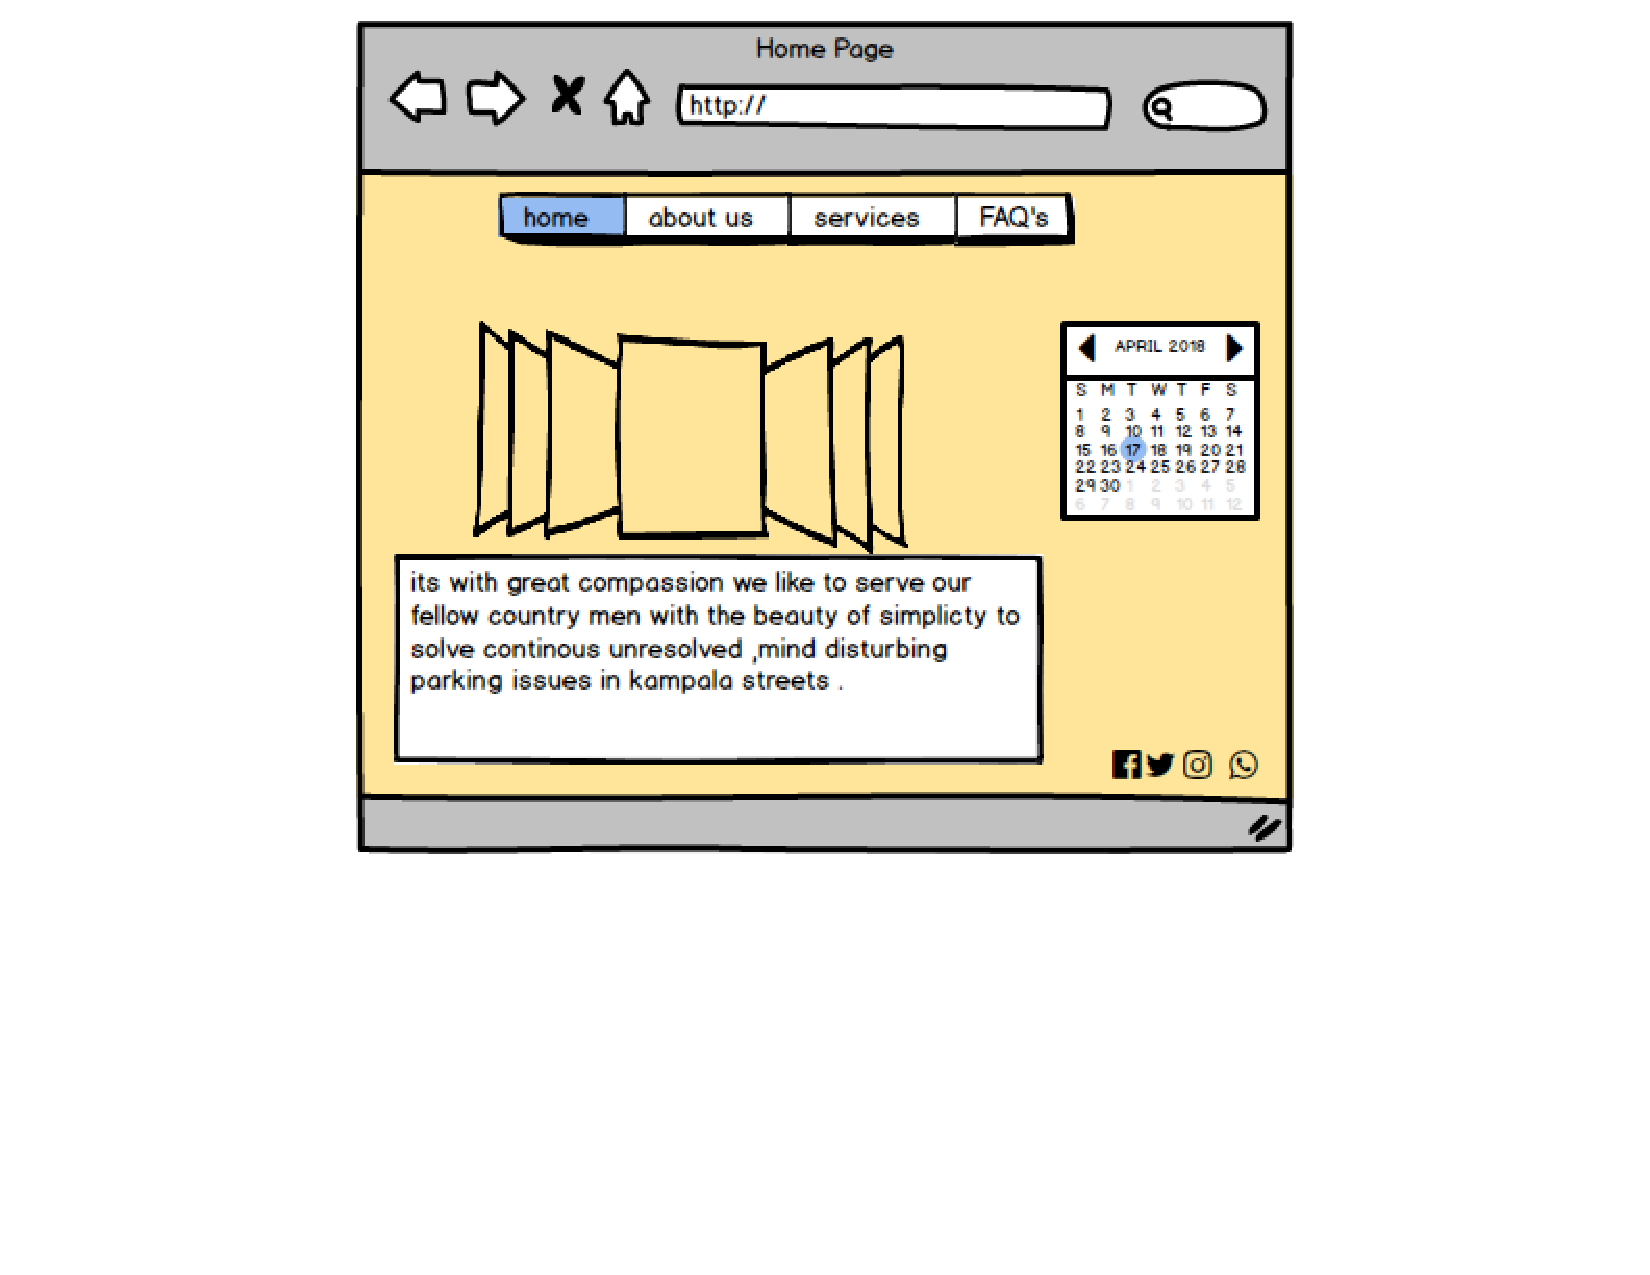
\includegraphics[width=\linewidth]{research.pdf}
     \caption{homepage.}
  \end{subfigure}
  \begin{subfigure}[b]{0.4\linewidth}
    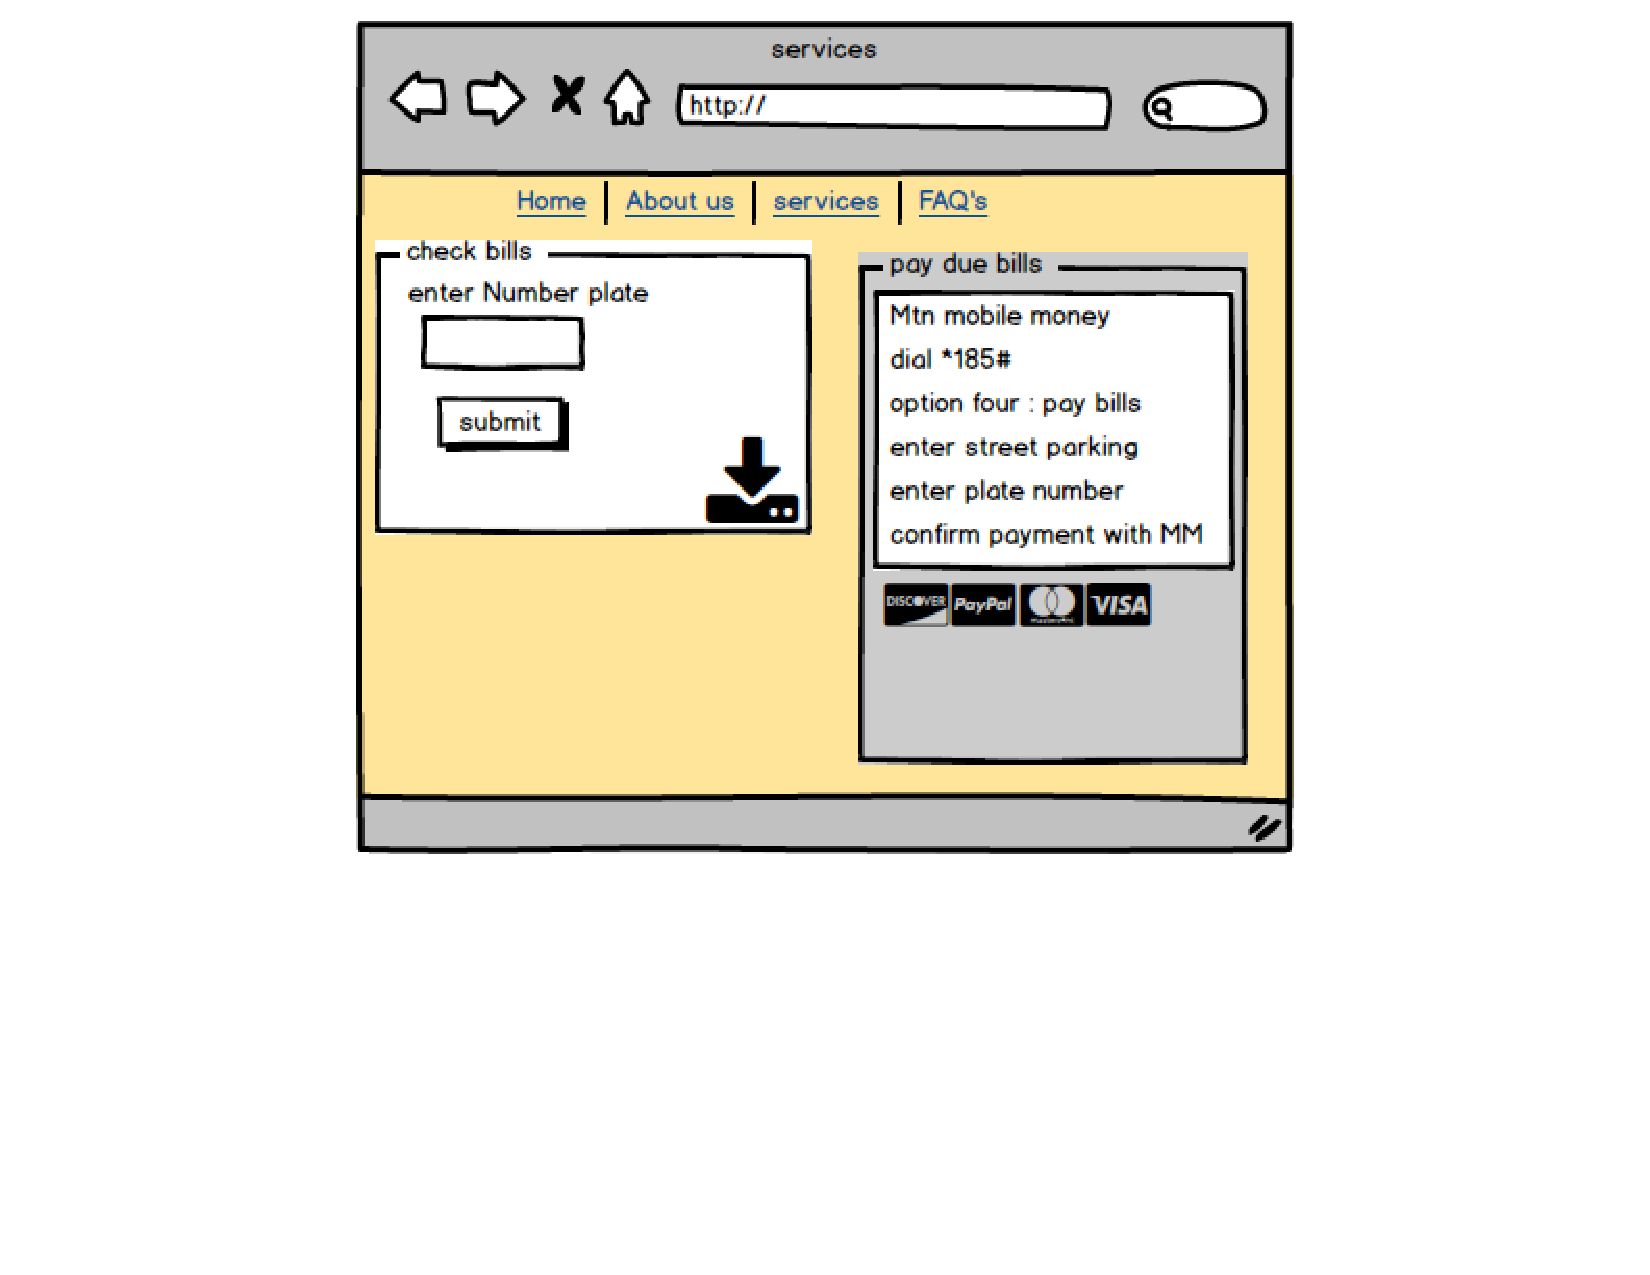
\includegraphics[width=\linewidth]{services.pdf}
    \caption{services page.}
  \end{subfigure}
  \begin{subfigure}[b]{0.4\linewidth}
    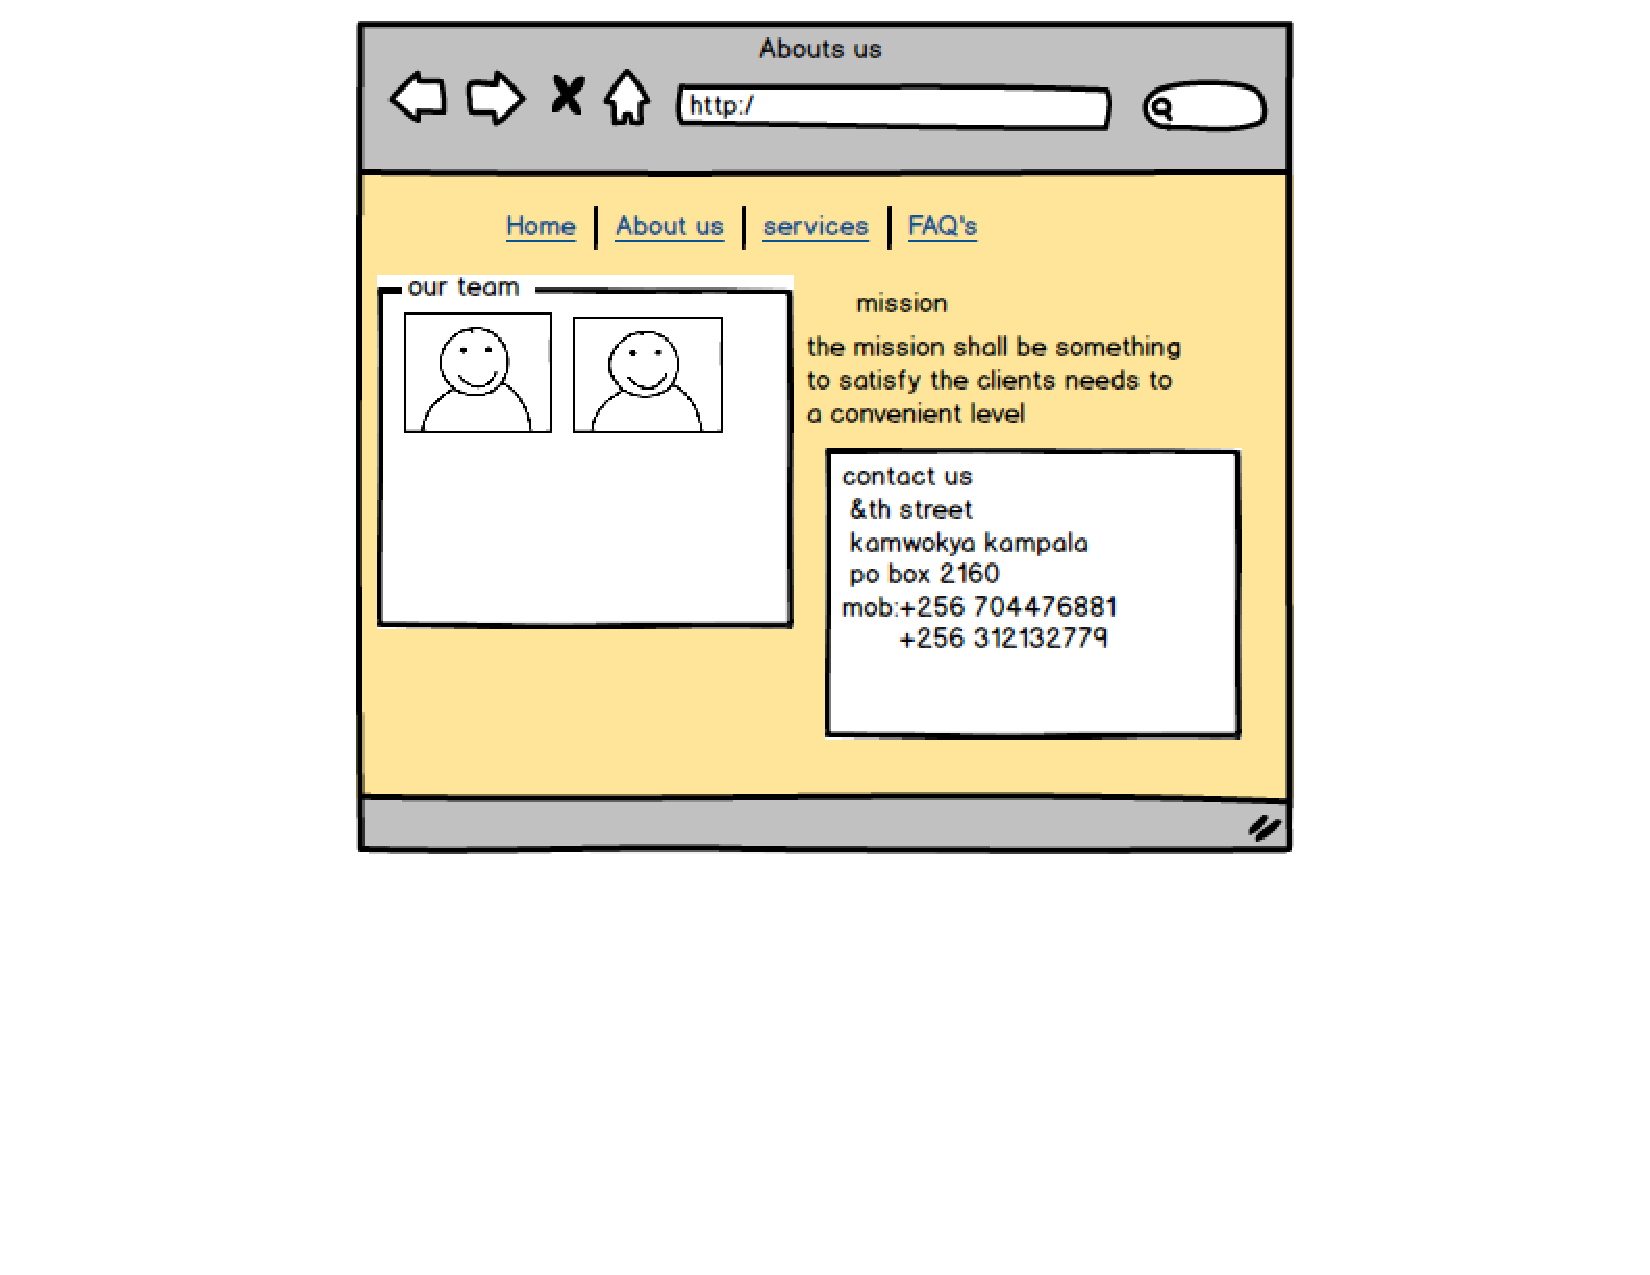
\includegraphics[width=\linewidth]{aboutus.pdf}
    \caption{about us page.}
  \end{subfigure}
  \begin{subfigure}[b]{0.4\linewidth}
    \includegraphics[width=\linewidth]{FAQ's.jpg}
    \caption{FAQ's.}
  \end{subfigure}
  \caption{user friendly display of interfaces.}
  \label{fig:3}
\end{figure}

\begin{figure}
  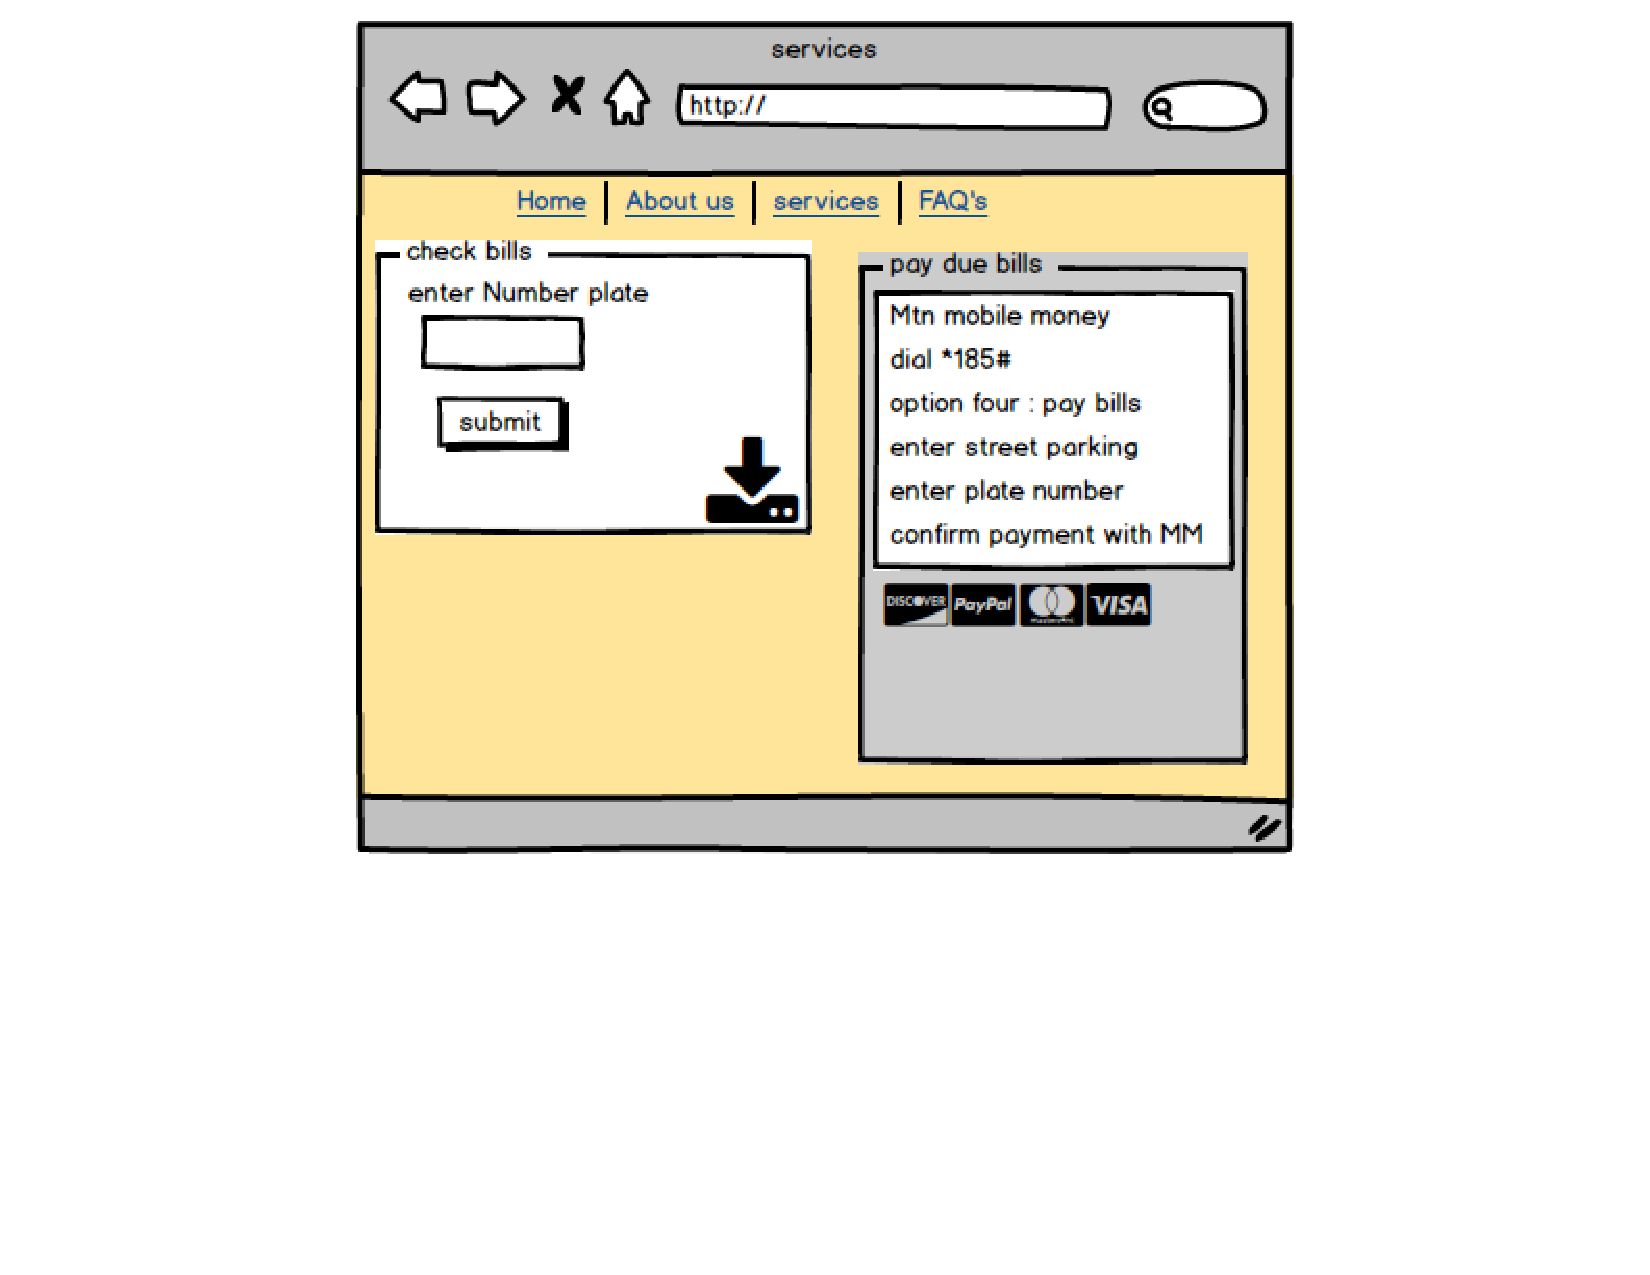
\includegraphics[width=\linewidth]{services.pdf}
 \caption{the core interface ,that will show a full display of the summarised generated report about parking bills , as well ease the settling of the bills with available payment options  }
  \end{figure} 

\newpage


\section{Appendices:\sc Selected terms and Recommended Readings}

\textbf {Survey}: refers to the method of securing information concerning a phenomena under study from all or a selected number of respondents to the concerned universe\\
\textbf {Touts}: refers to people writing tickets for cars parked on streets\\


1.C.R Kothari, Research Methodolgy Methods and techniques,University of Rajasthan,Jaipur(india).\\

2.Hellen Ntegyereize,Multiplex to automate street parking opeartions in kampala ,28-apr-2007 
 https://ugandaradionetwork.com/story/multiplex-to-automate-street-parking-operations-in-kampala\\

3.CAR PARKING SYSTEM BUILDING SOLUTION INTERNATIONAL 2158 Union Street, Simi Valley, CA-USA.\\ 
http://www.bsi-hardware.com/upload/download/20121119152338.pdf \\

4.Mayfield Handbook of Technical and ScientificWriting\\
 http://www.mhhe.com/mayfieldpub/tsw/pro-gen.htm

 








       


\end{document}